\documentclass[10pt,a4paper,twocolumn]{article}
\usepackage[utf8]{inputenc}
\usepackage[T1]{fontenc}
\usepackage{mathptmx}
\usepackage[provide=*]{babel}
\babelprovide[import,main]{french}
\usepackage[top=1.9cm,bottom=2.2cm,left=1.65cm,right=1.65cm,columnsep=0.6cm]{geometry}
\usepackage{graphicx}
\usepackage{booktabs}
\usepackage{enumitem}
\usepackage{titlesec}
\usepackage{caption}
\usepackage{microtype}
\usepackage{amsmath}
\usepackage[hidelinks]{hyperref}

\setlength{\parindent}{0.9em}
\setlength{\parskip}{0pt}
\renewcommand{\thesection}{\Roman{section}}
\renewcommand{\thesubsection}{\Alph{subsection}}
\titleformat{\section}{\centering\normalfont\small\scshape}{\thesection.}{0.5em}{}
\titleformat{\subsection}{\normalfont\itshape}{\thesubsection.}{0.5em}{}
\titlespacing*{\section}{0pt}{1.1ex plus 0.5ex}{0.8ex}
\titlespacing*{\subsection}{0pt}{1ex plus 0.4ex}{0.5ex}
\renewcommand{\thetable}{\Roman{table}}
\DeclareCaptionLabelFormat{up}{\scshape #1~#2}
\captionsetup{labelformat=up,labelsep=newline,font=footnotesize,justification=centering,singlelinecheck=false,
  skip=4pt}
\captionsetup[figure]{labelsep=period,justification=centering,name=Figure}
\captionsetup[table]{name=Table,textfont=scriptsize,labelfont=scriptsize}
\renewcommand{\figurename}{Figure}

\newcommand{\member}[1]{\begin{tabular}[t]{@{}c@{}}[Prénom NOM Postnom]\\ FASI, UPC\\ {[adresse@email.com]}\end{tabular}}

\begin{document}

\twocolumn[{%
\begin{center}
{\LARGE Rust, Go, PHP, Node.js ou Python : qui sert le mieux une même API de gestion de tâches ?\\[0.3ex]
\large Étude expérimentale de la performance sous charge}\\[1.4ex]
\small
\begin{tabular}{@{}cccc@{}}
\member{1}\hspace{1.2em} & \member{2}\hspace{1.2em} & \member{3}\hspace{1.2em} & \member{4}\\[1.2ex]
\end{tabular}\\
\begin{tabular}{@{}cc@{}}
\member{5}\hspace{4em} & \member{6}\\
\end{tabular}
\end{center}
\vspace{1ex}
}]

\noindent\textbf{\textit{Résumé}---}\textbf{\textit{Les affirmations sur la rapidité des langages de programmation
reposent rarement sur des mesures d'applications complètes. Nous comparons cinq implémentations équivalentes d'une
même API REST de gestion de tâches adossée à SQLite (Rust, Go, PHP, Node.js et Python) sous charge croissante (10, 50
et 100 utilisateurs simultanés), sur cinq fonctionnalités (création, liste paginée, recherche, jointure, statistiques).
Chaque cas est répété 30 fois, soit 2\,250 essais et 1,8 million de requêtes ; nous mesurons le débit, les latences
(médiane, p95, p99), le temps CPU par requête, la mémoire et le temps de démarrage. Sur les fonctionnalités légères,
Rust traite jusqu'à 9,3 fois plus de requêtes par seconde que Python (13\,373 contre 1\,433 en création) ; sur la
recherche et les statistiques, où SQLite domine, l'écart tombe à 1,5 et à environ 1. Ces résultats valent pour ces
implémentations, sur un seul cœur ; ils ne se généralisent pas aux langages.}}

\smallskip
\noindent\textit{\textbf{Mots-clés}---}performance, test de charge, API REST, SQLite, latence, Rust, Go, PHP, Node.js,
Python

\section{Introduction}
La performance d'une application web détermine l'attente de l'utilisateur, le nombre de serveurs à louer, la
consommation d'énergie et la capacité à absorber un pic de trafic. Elle intéresse donc autant les développeurs que
les équipes qui exploitent le service, notamment dans les contextes où le matériel et la bande passante sont
limités.

Des affirmations circulent pourtant sans mesure précise : « Rust est plus rapide que PHP », « Node.js tient mieux la
charge que Python ». Les travaux publiés comparent surtout des langages sur des programmes de calcul isolés
\cite{pereira2017}, alors qu'une application web passe l'essentiel de son temps à lire du réseau, à interroger une
base de données et à produire du JSON. La méthodologie de la mesure compte autant que le résultat : variabilité
entre exécutions, moyennes trompeuses, latences extrêmes \cite{georges2007,dean2013}, et même la configuration du
test peut fausser les données \cite{mytkowicz2009}.

\textbf{Question de recherche.} Pour une même API de gestion de tâches adossée à SQLite, de combien les
performances de cinq technologies (Rust, Go, PHP, Node.js, Python) diffèrent-elles, et cet écart dépend-il de la
fonctionnalité sollicitée et du nombre d'utilisateurs simultanés ?

\textbf{Hypothèses.}
\textbf{H1} : sur les fonctionnalités légères (créer, lister, jointure simple), l'ordre est Rust, Go, puis PHP et
Node.js, et enfin Python, car le coût propre à la technologie (analyse HTTP, JSON, interpréteur) domine.
\textbf{H2} : sur les fonctionnalités où SQLite travaille longtemps (recherche, agrégation), les écarts se réduisent,
car le temps est passé dans le moteur de base de données, identique pour toutes les versions.
\textbf{H3} : la latence extrême (p95, p99) croît avec la charge, et plus vite pour les technologies les moins
performantes.
\textbf{H4} : les versions compilées (Rust, Go) consomment moins de mémoire et démarrent plus vite que les versions
interprétées.

\textbf{Contribution et plan.} Nous présentons cinq implémentations équivalentes d'une même API, un protocole de
mesure répété 30 fois par cas et les données brutes associées. La section~\ref{sec:methodo} décrit la méthode, la
section~\ref{sec:dev} la réalisation, la section~\ref{sec:res} les résultats et leur discussion, puis nous
concluons.

\section{Méthodologie}\label{sec:methodo}
\subsection{Application de référence}
L'application est un gestionnaire de tâches (to-do) exposé comme une API REST en JSON. Les données sont
conservées dans SQLite : une table \texttt{categories} (20 lignes) et une table \texttt{tasks} (identifiant, titre,
description, statut parmi \textit{todo}/\textit{doing}/\textit{done}, priorité de 1 à 3, catégorie, échéance), avec
des index sur le statut et sur la catégorie. Toutes les versions partent de la même base de 10\,000 tâches, générée
avec une graine fixe. Cinq fonctionnalités sont soumises à la charge :
\textbf{F1} créer une tâche (écriture) ;
\textbf{F2} lister les tâches avec pagination (lecture et comptage) ;
\textbf{F3} rechercher par mot-clé (\texttt{LIKE}) avec filtre de statut facultatif (parcours de la table) ;
\textbf{F4} lister les tâches d'une catégorie (jointure) ;
\textbf{F5} calculer des statistiques par statut et par catégorie (agrégation).
Trois routes complètent le CRUD (lire, modifier le statut, supprimer) ; elles sont vérifiées par le test
d'équivalence mais ne sont pas chargées. Le cahier des charges complet (routes, validations, codes d'erreur) est joint
au rendu.

\subsection{Technologies comparées}
Nous comparons cinq technologies (tableau~\ref{tab:techs}), qui couvrent plusieurs modèles d'exécution : code natif
compilé (Rust, Go), JavaScript compilé à la volée sur une boucle d'événements (Node.js) et langages interprétés
(PHP, Python). PHP et Python sont aussi des langages très répandus pour le développement web, ce qui rend
la comparaison utile aux étudiants. Chaque version utilise le serveur HTTP le plus simple disponible dans sa
technologie, sans paquet externe (voir la section~\ref{sec:dev}).

\begin{table}[t]
\caption{Technologies comparées}\label{tab:techs}
\centering\small
\begin{tabular}{@{}llll@{}}
\toprule
\textbf{Technologie} & \textbf{Langage} & \textbf{Version} & \textbf{SQLite}\\
\midrule
Flask 3.1.3 & Python & 3.13.18 & 3.53.1\\
module \texttt{http} & Node.js & 22.23.4 & 3.53.4\\
\texttt{php -S} & PHP & 8.3.6 & 3.45.1\\
\texttt{net/http} & Go & 1.24.7 & 3.45.1\\
bibl. standard & Rust & 1.97.0 & 3.45.1\\
\bottomrule
\end{tabular}
\end{table}

\subsection{Métriques}
Une seule grandeur ne suffit pas pour dire qu'une version est « plus performante » : un serveur peut répondre vite
en consommant beaucoup de processeur, ou tenir la charge en répondant lentement à certains utilisateurs. Nous
retenons six familles de mesures, relevées pour chaque essai.
\begin{itemize}[leftmargin=*,itemsep=0pt,topsep=2pt]
\item \textbf{Débit} (requêtes/s) : nombre de requêtes traitées divisé par la durée de l'essai ; mesure la capacité
à absorber du trafic. Outil : générateur de charge.
\item \textbf{Latence moyenne, médiane (p50), p95 et p99} (ms) : durée entre l'envoi de la requête et la fin de la
réponse, vue par le client. La médiane décrit le cas courant, p95 et p99 l'expérience des utilisateurs les moins
bien servis, que la moyenne masque \cite{dean2013}.
\item \textbf{Taux d'erreur} : requêtes échouées (réseau ou code HTTP hors 2xx) ; un débit n'a de sens que sans erreur.
\item \textbf{Temps CPU par requête} (ms) : temps processeur (utilisateur + système) du serveur pendant l'essai,
divisé par le nombre de requêtes ; mesure le coût de chaque requête, donc l'efficacité énergétique et financière.
Outil : \texttt{psutil}, d'après \texttt{/proc}.
\item \textbf{Mémoire} (Mo) : \textit{proportional set size} (PSS) de tous les processus du serveur en fin d'essai
(plus fidèle que la RSS lorsque plusieurs processus partagent des pages, comme PHP).
\item \textbf{Temps de démarrage} (ms) : du lancement du processus à la première réponse correcte ; utile pour
le déploiement et la mise à l'échelle.
\end{itemize}

\subsection{Outils et environnement de test}
Le générateur de charge est un programme Go écrit pour l'occasion (aucun outil comme k6 ou wrk n'était disponible
sur la machine, sans accès réseau). Chaque « utilisateur simultané » est une goroutine qui garde sa connexion HTTP/1.1
ouverte et envoie la requête suivante dès la réponse reçue (boucle fermée, sans temps de réflexion \cite{jain1991}). Les tests
s'exécutent dans un conteneur Linux (Ubuntu 24.04, noyau 6.18) à 2 cœurs virtuels (Xeon à 2,1\,GHz) et 8\,Go de
mémoire. Le serveur est épinglé sur le cœur~0 et le générateur sur le cœur~1 (\texttt{taskset}), si bien que
\emph{chaque version dispose d'un seul cœur} : les résultats mesurent le rendement par cœur, non l'avantage du
parallélisme.

\subsection{Déroulement des tests}
Pour chaque fonctionnalité (F1 à F5), chaque niveau de charge (10, 50 et 100 utilisateurs simultanés) et chaque
essai numéroté de 1 à 30, nous exécutons, pour les cinq technologies dans un ordre tiré au sort (graine fixe) :
(1)~copie d'une base neuve identique et démarrage du serveur ; (2)~100 requêtes de chauffe, non comptées ;
(3)~essai mesuré de 1\,000 requêtes (500 pour F3 et F5, plus longues) réparties entre les utilisateurs ;
(4)~relevé du CPU et de la mémoire, puis arrêt du serveur. L'ordre aléatoire répartit sur toutes les technologies
les dérives de la machine (cache, voisins du conteneur) ; le redémarrage à chaque essai rend les essais
indépendants, y compris pour F1 qui modifie la base. Les 30 essais par cas permettent de calculer des moyennes
avec intervalles de confiance à 95\,\% et des tests de comparaison \cite{georges2007}.
Les scripts, le générateur et les données brutes sont fournis pour répéter l'expérience.

\section{Développement}\label{sec:dev}
\subsection{Réalisation des versions}
Les cinq versions, les scripts de test et le programme d'analyse ont été produits avec l'assistance d'un outil
d'intelligence artificielle (Claude, d'Anthropic), ce que l'énoncé du travail autorise. Chaque version reprend la
même structure : un routeur, la validation des entrées, des requêtes SQL identiques et la construction de la réponse
JSON. Toutes utilisent le mode WAL de SQLite \cite{sqlitewal}, quatre connexions à la base (une seule pour Node.js, dont le code
s'exécute dans un seul fil) et des connexions HTTP persistantes.
\begin{itemize}[leftmargin=*,itemsep=0pt,topsep=2pt]
\item \textbf{Python} : Flask, avec le serveur de développement de Werkzeug en mode multifil (HTTP/1.1) et le module
\texttt{sqlite3} ;
\item \textbf{Node.js} : module \texttt{http} natif et \texttt{node:sqlite}, requêtes préparées une fois ;
\item \textbf{PHP} : serveur intégré \texttt{php -S} avec quatre processus de travail, PDO SQLite à connexion persistante ;
\item \textbf{Go} : \texttt{net/http} et un accès SQLite écrit avec cgo (liaison à \texttt{libsqlite3}) ;
\item \textbf{Rust} : bibliothèque standard seulement : serveur HTTP/1.1 minimal à un fil par connexion, lecteur
JSON écrit à la main et appels FFI à \texttt{libsqlite3}.
\end{itemize}
La machine n'ayant pas d'accès au réseau, les frameworks cités dans l'énoncé à titre d'exemple (Axum, Express,
Laravel) n'ont pas pu être installés. Cela signifie que les versions Go et Rust utilisent un serveur plus
rudimentaire que celui d'un projet réel, et que Python (Flask) est la seule version bâtie sur un framework.

\subsection{Équivalence fonctionnelle}
L'équivalence est vérifiée par un scénario de 69 requêtes rejoué sur chaque version, à partir d'une base neuve : 26
réponses 200, 3 créations (dont un titre avec accents, guillemets et caractères japonais), 1 suppression, 26 erreurs
400 (JSON invalide, statut ou priorité hors domaine, page ou limite non numérique, clé étrangère inexistante,
titre de 201 caractères) et 13 erreurs 404. Pour chaque requête, le code HTTP et le corps JSON analysé sont comparés.
Les cinq versions donnent exactement les mêmes réponses sur les 69 requêtes. Pendant les essais de charge, les
codes de réponse sont aussi contrôlés : le nombre total d'erreurs est indiqué dans la section~\ref{sec:res}.

\subsection{Difficultés rencontrées}
\emph{Versions de SQLite.} Python et Node.js embarquent leur propre SQLite (3.53), alors que PHP, Go et Rust utilisent
la bibliothèque du système (3.45.1). Cet écart n'a pas pu être supprimé ; il est une limite de l'étude (section IV-C).
\emph{Représentation du JSON en Go.} Une première version Go construisait des \texttt{map} génériques ; son débit
sur F2 était plus faible. Remplacer ces \texttt{map} par des structures typées a rendu l'implémentation plus
idiomatique, et l'équivalence a été revérifiée.
\emph{Serveurs « de développement ».} Le serveur Werkzeug de Flask et \texttt{php -S} sont déconseillés en production ;
les résultats de Python et PHP concernent donc cette configuration, non un déploiement avec Gunicorn ou
PHP-FPM.
\emph{Connexions persistantes.} Flask répond en HTTP/1.0 par défaut ; nous avons forcé HTTP/1.1 pour que toutes les
versions réutilisent leurs connexions.

\section{Résultats et discussion}\label{sec:res}
\subsection{Données recueillies}
La campagne comprend 2\,250 essais (5 technologies $\times$ 5 fonctionnalités $\times$ 3 niveaux de charge $\times$
30 essais), soit 1,8 million de requêtes mesurées et 225\,000 requêtes de chauffe. Aucune requête n'a échoué. Le
fichier brut contient une ligne par essai (18 colonnes : débit, latences, CPU, mémoire, démarrage). D'un essai à
l'autre, le débit varie en médiane de 9,7\,\% (écart-type rapporté à la moyenne) et jusqu'à 17,6\,\% : les écarts
inférieurs à environ 15\,\% ne se lisent donc pas sur un essai isolé, et les comparaisons ci-dessous reposent sur
les 30 essais (test de Mann-Whitney deux à deux, correction de Holm). Sauf mention contraire, les valeurs sont
données pour 50 utilisateurs simultanés.

\begin{table}[t]
\caption{Débit moyen (requêtes/s) à 50 utilisateurs, 30 essais par case}\label{tab:debit}
\centering\small
\begin{tabular}{@{}lrrrrr@{}}
\toprule
\textbf{Techno.} & \textbf{F1} & \textbf{F2} & \textbf{F3} & \textbf{F4} & \textbf{F5}\\
\midrule
Rust & 13\,373 & 7\,735 & 806 & 9\,261 & 243 \\
Go & 7\,517 & 5\,820 & 761 & 6\,791 & 237 \\
PHP & 6\,488 & 5\,500 & 721 & 6\,335 & 230 \\
Node.js & 4\,792 & 4\,003 & 752 & 4\,186 & 271 \\
Python & 1\,433 & 1\,443 & 535 & 1\,468 & 242 \\
\bottomrule
\end{tabular}
\end{table}

\begin{table}[t]
\caption{Latence, CPU, mémoire et démarrage (50 utilisateurs)}\label{tab:synth}
\centering\small
\setlength{\tabcolsep}{3.5pt}
\begin{tabular}{@{}lrrrrr@{}}
\toprule
 & \textbf{p95 F2} & \textbf{CPU F1} & \textbf{CPU F5} & \textbf{Mém.} & \textbf{Démar.}\\
\textbf{Techno.} & {\scriptsize(ms)} & {\scriptsize(ms/req)} & {\scriptsize(ms/req)} & {\scriptsize(Mo)} & {\scriptsize(ms)}\\
\midrule
Rust & 11,1 & 0,06 & 4,08 & 9 & 6 \\
Go & 15,9 & 0,11 & 4,18 & 18 & 7 \\
PHP & 23,2 & 0,13 & 4,29 & 42 & 30 \\
Node.js & 22,3 & 0,18 & 3,67 & 53 & 41 \\
Python & 40,8 & 0,68 & 4,11 & 33 & 160 \\
\bottomrule
\end{tabular}
\end{table}

\subsection{Analyse}
\paragraph{Débit.} La figure~\ref{fig:debit} et le tableau~\ref{tab:debit} montrent un classement net sur les
fonctionnalités légères. En création (F1), Rust traite 13\,373 requêtes/s (intervalle de confiance à 95\,\% :
$\pm$567), contre 7\,517 pour Go, 6\,488 pour PHP, 4\,792 pour Node.js et 1\,433 pour Python : Rust est 9,3 fois plus
rapide que Python. Les rapports Rust/Python sont de 5,4 en liste (F2) et de 6,3 en jointure (F4). Les dix paires de
technologies diffèrent significativement pour F1, F2 et F4. Pour la recherche (F3), l'écart se réduit à 1,5 entre
Rust (806) et Python (535), et Go et PHP ne se distinguent pas statistiquement de Node.js (Go--Node.js :
$p=0{,}51$ ; PHP--Node.js : $p=0{,}07$). Pour les statistiques (F5), les cinq versions se situent entre 230 et
271 requêtes/s ; Rust et Python sont indiscernables ($p=0{,}68$) et Node.js est de 12 à 18\,\% au-dessus des autres.

\begin{figure}[t]
\centering
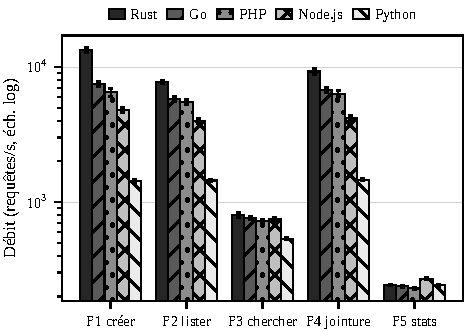
\includegraphics[width=\columnwidth]{figures/fig_debit.pdf}
\caption{Débit par fonctionnalité à 50 utilisateurs (barres : intervalle de confiance à 95\,\%, 30 essais).}
\label{fig:debit}
\end{figure}

\paragraph{Évolution avec la charge.} Le débit reste presque constant de 10 à 100 utilisateurs (par exemple Python
en F1 : 1\,445, 1\,433 et 1\,450 requêtes/s) : le cœur du serveur est déjà saturé dès 10 utilisateurs. Comme les
utilisateurs envoient une requête dès la réponse reçue, la latence moyenne vaut à peu près le nombre d'utilisateurs
divisé par le débit (loi de Little) et croît donc proportionnellement. La latence p95 de F1 (figure~\ref{fig:charge1})
passe de 12,9 à 80,0\,ms pour Python (+67\,ms) et de 1,9 à 17,8\,ms pour Rust (+16\,ms) entre 10 et 100 utilisateurs.

\begin{figure}[t]
\centering
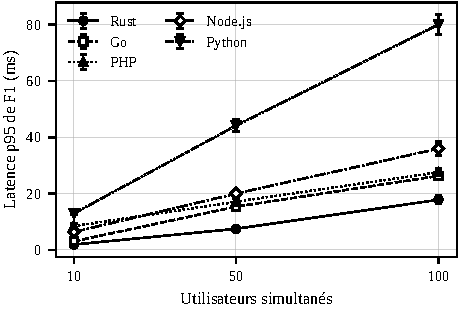
\includegraphics[width=\columnwidth]{figures/fig_charge_create.pdf}
\caption{Latence p95 de la création (F1) selon le nombre d'utilisateurs simultanés.}
\label{fig:charge1}
\end{figure}

\paragraph{Latences extrêmes.} En F5, les latences médianes des cinq versions sont proches (175 à 210\,ms), mais la
latence p95 de Rust atteint 396\,ms, contre 215 à 275\,ms pour les autres (figure~\ref{fig:charge5}). À 100
utilisateurs, elle est de 846\,ms pour Rust et de 405 à 577\,ms pour les autres. Une moyenne seule aurait caché cette
différence.

\begin{figure}[t]
\centering
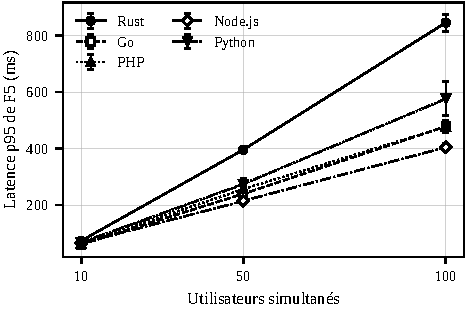
\includegraphics[width=\columnwidth]{figures/fig_charge_stats.pdf}
\caption{Latence p95 des statistiques (F5) selon le nombre d'utilisateurs simultanés.}
\label{fig:charge5}
\end{figure}

\paragraph{Coût en processeur.} La figure~\ref{fig:cpu} montre le temps CPU consommé par requête. En F1, Python
dépense 0,68\,ms, soit 11 fois plus que Rust (0,06\,ms), Go (0,11), PHP (0,13) et Node.js (0,18) se situant entre les
deux. En F3 et F5, ce coût est de 1,2 à 1,8\,ms et de 3,7 à 4,3\,ms pour toutes les versions : l'essentiel est
dépensé par SQLite.

\begin{figure}[t]
\centering
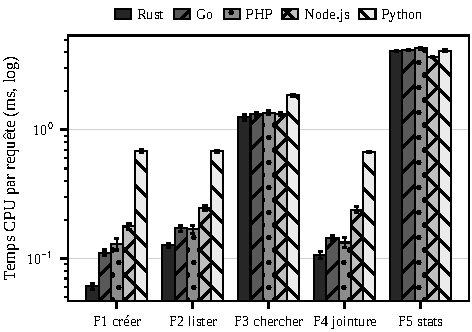
\includegraphics[width=\columnwidth]{figures/fig_cpu.pdf}
\caption{Temps CPU du serveur par requête, à 50 utilisateurs (échelle logarithmique).}
\label{fig:cpu}
\end{figure}

\paragraph{Mémoire et démarrage.} Rust occupe 8,5\,Mo et démarre en 6\,ms, Go 17,6\,Mo et 7\,ms. Python (33,5\,Mo,
160\,ms), PHP (41,7\,Mo pour ses cinq processus, 30\,ms) et Node.js (52,9\,Mo, 41\,ms) viennent ensuite
(figure~\ref{fig:mem}, tableau~\ref{tab:synth}).

\begin{figure}[t]
\centering
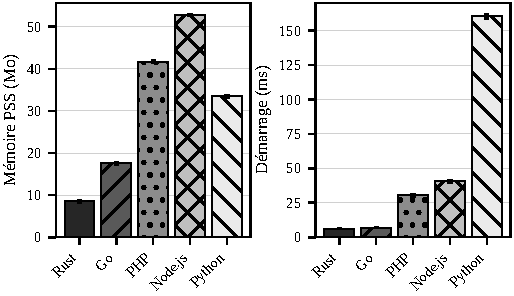
\includegraphics[width=0.92\columnwidth]{figures/fig_memoire_demarrage.pdf}
\caption{Mémoire (PSS en fin d'essai) et temps de démarrage, moyennes sur tous les essais.}
\label{fig:mem}
\end{figure}

\subsection{Interprétation et discussion}
\textbf{H1 est confirmée en grande partie.} Sur F1, F2 et F4, l'ordre Rust, Go, PHP, Node.js, Python est respecté et
chaque paire est significativement différente. Notre hypothèse plaçait pourtant PHP et Node.js au même niveau : PHP
est en réalité meilleur (par exemple 6\,488 contre 4\,792 requêtes/s en F1), avec un coût CPU par requête plus faible
(0,13 contre 0,18\,ms). Nous n'avons pas isolé la cause ; l'hypothèse la plus simple est que le chemin d'une requête
(analyse HTTP, décodage de l'URL, JSON) est plus court dans le serveur intégré de PHP, écrit en C, que dans les
couches JavaScript de Node.js.

\textbf{H2 est confirmée.} En F5, le CPU mesuré par requête (3,7 à 4,3\,ms) est proche du temps des deux requêtes SQL
exécutées seules, sans HTTP : 3,4\,ms dans Node.js (SQLite 3.53.4), 3,7 dans Python (3.53.1) et 4,2 dans PHP
(3.45.1). Le surcoût propre à la technologie ne représente que quelques dixièmes de milliseconde. Le léger avantage
de Node.js en F5 est cohérent avec un moteur SQLite plus récent, mais Python a la même version 3.53 sans cet avantage
et nous ne pouvons pas séparer les deux effets.

\textbf{H3 est partiellement confirmée.} La latence extrême croît bien avec la charge pour toutes les versions, et
l'augmentation absolue est la plus forte pour Python. En valeur relative, c'est pourtant Rust qui varie le plus (la
p95 de F1 est multipliée par 9,4, contre 6,2 pour Python), car sa latence à faible charge est très petite. Pour la
p95 de F5, Rust est le moins bon : nous supposons que les 50 fils d'exécution se disputent les quatre connexions
SQLite sans ordre d'attente équitable (verrou et variable de condition), mais ce point n'a pas été vérifié.

\textbf{H4 est partiellement confirmée.} Rust et Go sont les moins gourmands et les plus rapides au démarrage, mais
les technologies interprétées ne sont pas toutes plus lourdes : Python consomme moins de mémoire que PHP et Node.js.

\textbf{Portée.} Un facteur 9 n'a d'effet que si le serveur est saturé : à 1\,433 requêtes/s, la version Python sert
déjà, à titre d'ordre de grandeur, plus de 100 millions de requêtes par jour sur un seul cœur. Dès que SQLite travaille
(F3, F5), changer de langage apporte peu : l'effort doit alors porter sur la requête et l'index.

\textbf{Limites.} (i)~Nous comparons cinq implémentations, pas cinq langages : les versions Go et Rust utilisent
un serveur rudimentaire, et Flask et \texttt{php -S} sont des serveurs de développement. (ii)~Chaque serveur est limité
à un cœur ; le gain du parallélisme n'est pas mesuré. (iii)~Les versions de SQLite diffèrent (3.53 pour Python et
Node.js, 3.45.1 pour les autres). (iv)~Le client et le serveur communiquent sur la même machine, sans réseau, dans un
conteneur partagé à deux cœurs : les valeurs absolues ne se transposent pas à une autre machine, seules leurs
proportions sont instructives. (v)~La base (10\,000 lignes) tient en mémoire et chaque essai compte 500 ou 1\,000
requêtes. (vi)~Nous n'avons pas testé d'autres frameworks ni d'autres bases de données.

\section{Conclusion}
Nous voulions savoir de combien les performances de cinq technologies diffèrent pour une même API de gestion de
tâches. La réponse dépend de la fonctionnalité : sur les opérations légères, Rust traite de 5 à 9 fois plus de
requêtes par seconde que Python, avec un coût CPU par requête jusqu'à 11 fois plus faible, et l'ordre Rust, Go, PHP,
Node.js, Python est stable ; sur les opérations dominées par SQLite, les cinq versions se rapprochent, car le moteur
de base de données est le même. Rust et Go ont aussi l'empreinte mémoire la plus faible et démarrent en quelques
millisecondes. Les moyennes ne suffisent pas : la latence p95 de Rust sur les statistiques est la plus mauvaise malgré
une médiane comparable.

Ces résultats ont des limites : un seul cœur, des serveurs simples ou de développement, deux versions de SQLite, une
seule machine partagée. Une suite naturelle serait de reprendre l'étude avec les frameworks usuels (Axum, Express,
Laravel, Django) et des serveurs de production, de laisser chaque version utiliser tous les cœurs, d'utiliser une
base client-serveur comme PostgreSQL, et de vérifier l'explication proposée pour la latence extrême de Rust.


\renewcommand{\refname}{\centering\normalfont\small\scshape Références}
\begin{thebibliography}{9}\footnotesize
\setlength{\itemsep}{0pt}
\bibitem{pereira2017} R. Pereira, M. Couto, F. Ribeiro, R. Rua, J. Cunha, J. P. Fernandes et J. Saraiva,
« Energy efficiency across programming languages: how do energy, time, and memory relate? », \textit{Proc. 10th ACM
SIGPLAN Int. Conf. on Software Language Engineering (SLE)}, ACM, 2017. DOI : 10.1145/3136014.3136031.
\bibitem{georges2007} A. Georges, D. Buytaert et L. Eeckhout, « Statistically rigorous Java performance evaluation »,
\textit{Proc. OOPSLA 2007}, ACM, p. 57--76, 2007.
\bibitem{dean2013} J. Dean et L. A. Barroso, « The tail at scale », \textit{Communications of the ACM}, vol. 56,
no 2, p. 74--80, 2013.
\bibitem{mytkowicz2009} T. Mytkowicz, A. Diwan, M. Hauswirth et P. F. Sweeney, « Producing wrong data without doing
anything obviously wrong! », \textit{Proc. ASPLOS XIV}, ACM, p. 265--276, 2009.
\bibitem{jain1991} R. Jain, \textit{The Art of Computer Systems Performance Analysis}. New York : Wiley, 1991.
\bibitem{sqlitewal} SQLite, « Write-Ahead Logging », 2026. [En ligne]. Disponible : https://www.sqlite.org/wal.html.
[Consulté le 15 novembre 2026].
\end{thebibliography}

\end{document}
